% related_work.tex
\section{Related Work}
\label{sec:related}

% Framework figure - placed early so it appears at top of page 3
\begin{figure*}[!t]
    \centering
    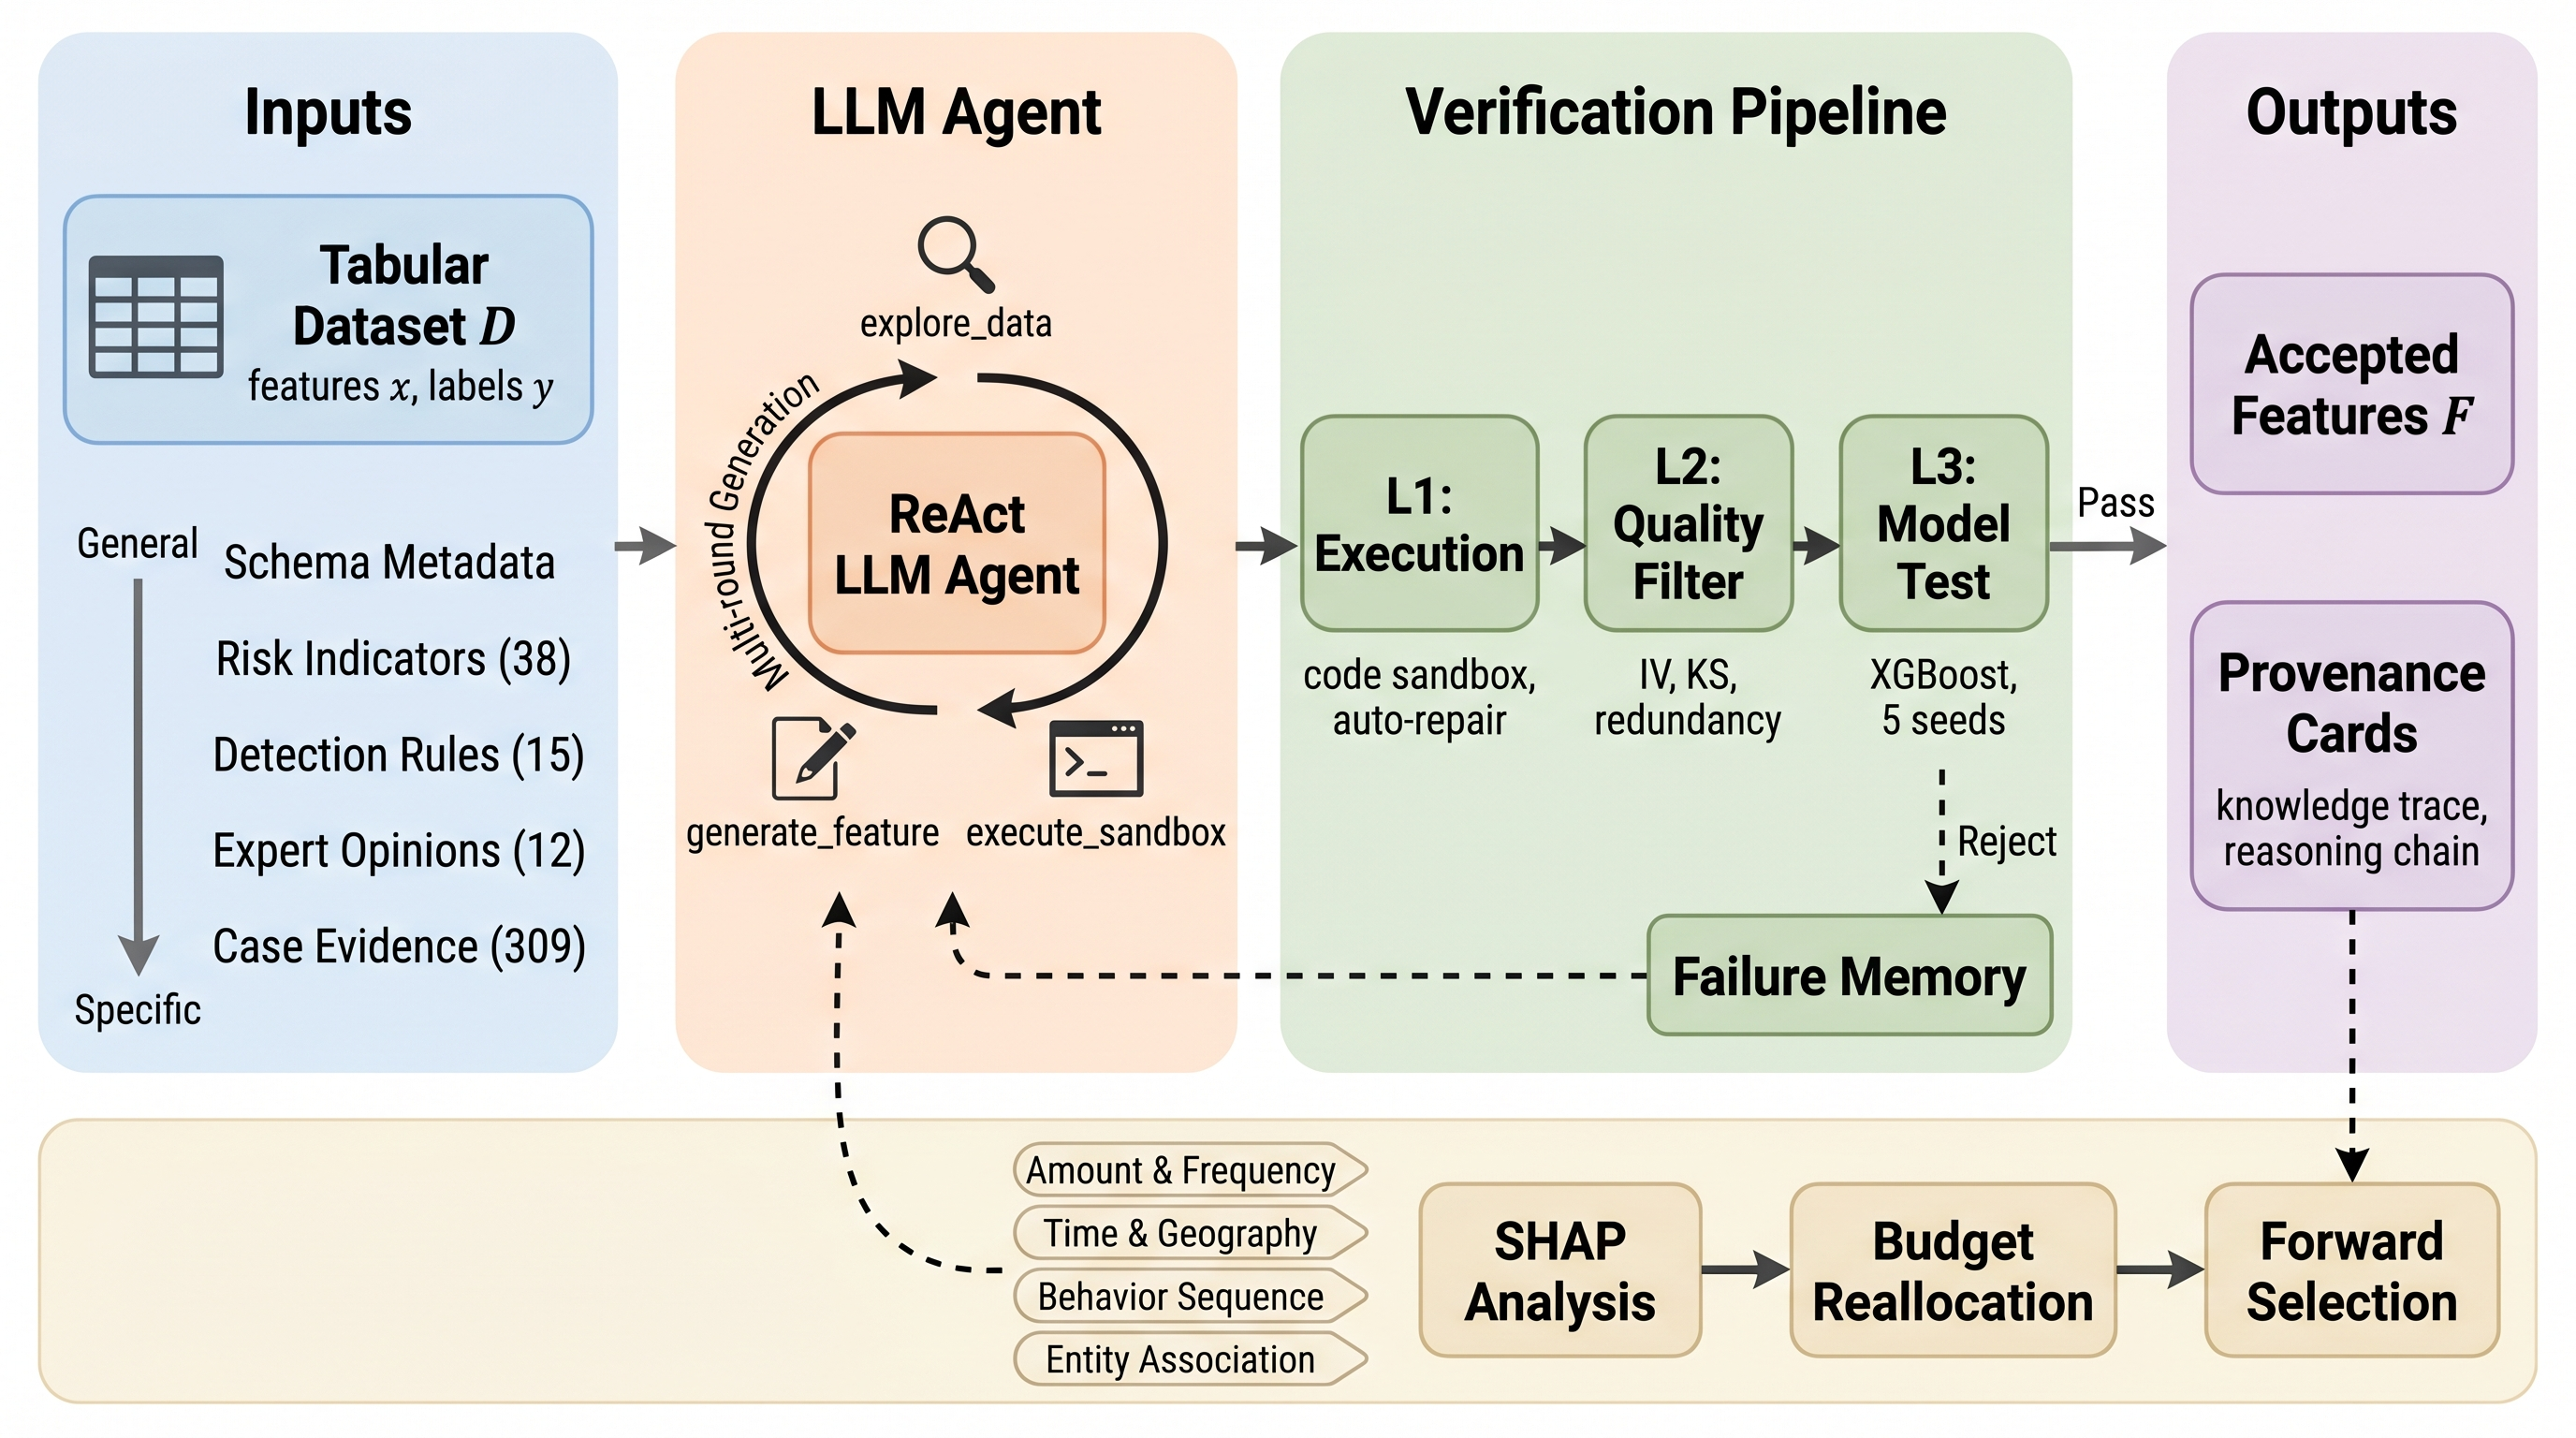
\includegraphics[width=0.85\textwidth]{figures/framework.png}
    \caption{Overview of the KnowFeat framework. Color coding: blue = inputs (data \& knowledge), yellow = core LLM agent, green = verification pipeline (L1--L3), purple = outputs (features \& provenance cards), gray = SHAP-guided search strategy. The agent generates features grounded in hierarchical domain knowledge; each candidate is verified through a three-stage pipeline; SHAP feedback dynamically reallocates the exploration budget across semantic dimensions.}
    \label{fig:framework}
\end{figure*}

\subsection{Automated Feature Engineering}

Traditional AutoFE methods search a \emph{syntactic} transformation space. Deep Feature Synthesis~\cite{kanter2015deep} applies aggregation primitives along relational paths; ExploreKit~\cite{katz2016explorekit} enumerates operators via meta-learning; AutoFeat~\cite{horn2019autofeat} uses polynomial expansion with L1 selection; and OpenFE~\cite{zhang2023openfe} frames generation as operator-operand search with LightGBM-based ranking. AutoML systems such as Auto-sklearn~\cite{feurer2015auto} and FLAML~\cite{wang2021flaml} include preprocessing but do not generate semantically new features. These methods apply predefined operators without \emph{semantic} understanding~\cite{nargesian2017learning}.

The emergence of LLMs~\cite{brown2020gpt3,touvron2023llama} enabled semantic feature generation. CAAFE~\cite{hollmann2023caafe} iteratively prompts an LLM to generate Python code using logistic regression feedback. FeatLLM~\cite{han2024featllm} extracts rules and converts them to binary indicators. LLM-FE~\cite{abhyankar2025llmfe} uses evolutionary optimization with model performance feedback. RiskTagger~\cite{li2025risktagger} uses regulatory knowledge for Web3 behavior annotation. Tool-augmented agents~\cite{yao2023react} have been applied to code generation~\cite{qian2024chatdev}, software engineering~\cite{jimenez2024swe}, and data science~\cite{hong2024data,jiang2025aide,guo2024ds}, but none addresses knowledge-grounded feature generation.

These methods vary in domain knowledge and verification depth. Table~\ref{tab:comparison} summarizes the key differences. KnowFeat is the first to combine hierarchical structured knowledge, multi-stage verification (L1--L3), and full provenance tracking.

In financial AML, domain experts manually encode risk indicators and network measures~\cite{chen2018aml}, regulatory bodies publish red-flag typologies~\cite{fatf2012recommendations}, and institutions maintain detection rules from compliance experience~\cite{weber2019anti}. Knowledge-infused learning~\cite{kursuncu2020knowledge} and transfer learning~\cite{weiss2016survey} target unstructured data rather than tabular features. This rich, structured AML knowledge has not been systematically leveraged by automated feature engineering.

\begin{table}[t]
\centering
\caption{Comparison of automated feature engineering methods. \checkmark: fully supported; $\circ$: partially supported; blank: not supported; --: not applicable.}
\label{tab:comparison}
\small
\renewcommand{\arraystretch}{1.2}
\setlength{\tabcolsep}{1pt}
\begin{tabular}{l c c c c c c c}
\hline
\textbf{Property} & \textbf{OpenFE} & \textbf{AutoF.} & \textbf{CAAFE} & \textbf{FeatL.} & \textbf{LLM-FE} & \textbf{RiskT.} & \textbf{Ours} \\
\hline
Semantic underst. &            &            & \checkmark & \checkmark & \checkmark & \checkmark & \checkmark \\
Hier.\ knowledge  &            &            &            &            & $\circ^1$    & $\circ^2$    & \checkmark \\
Exec.\ verific.   & --         & --         &            &            &            &            & \checkmark \\
Statistical filt. & \checkmark & \checkmark &            &            &            &            & \checkmark \\
Model validation  &            &            & $\circ^3$       &            & \checkmark &            & \checkmark \\
Provenance track. &            &            &            &            &            & $\circ^4$    & \checkmark \\
Adaptive search   &            &            &            &            & \checkmark &            & \checkmark \\
\hline
\multicolumn{8}{l}{\scriptsize $^1$Dataset desc.\ only. $^2$Regulatory guidelines only. $^3$LogReg proxy. $^4$NL rationales only.} \\
\end{tabular}
\end{table}
